% !TEX root = ./article.tex

\documentclass{article}

\usepackage{mystyle}
\usepackage{myvars}



%-----------------------------

\begin{document}

	\maketitle % Insert title

	\thispagestyle{fancy} % All pages have headers and footers


%-----------------------------
%	ABSTRACT
%-----------------------------

	\begin{abstract}
		\noindent [TODO ]
	\end{abstract}

%-----------------------------
%	TEXT
%-----------------------------


	\section{Introducción}
	\label{sec:introducción}

		\paragraph{}
		[TODO]

	\section{La figura \ref{e1:plot} muestra un conjunto de entrenamiento con ejemplos positivos (estrellas) y negativos (círculos). Se desea clasificar la nueva instancia $<3,3>$ mediante el algoritmo $K$-vecinos más próximos. Obtener la clasificación para los valores de $K=\{ 1, 3, 5\}$ utilizando las distancias indicadas a continuación}
	\label{sec:e1}

		\paragraph{}
		[TODO]

		\begin{figure}[h]
			\begin{center}
				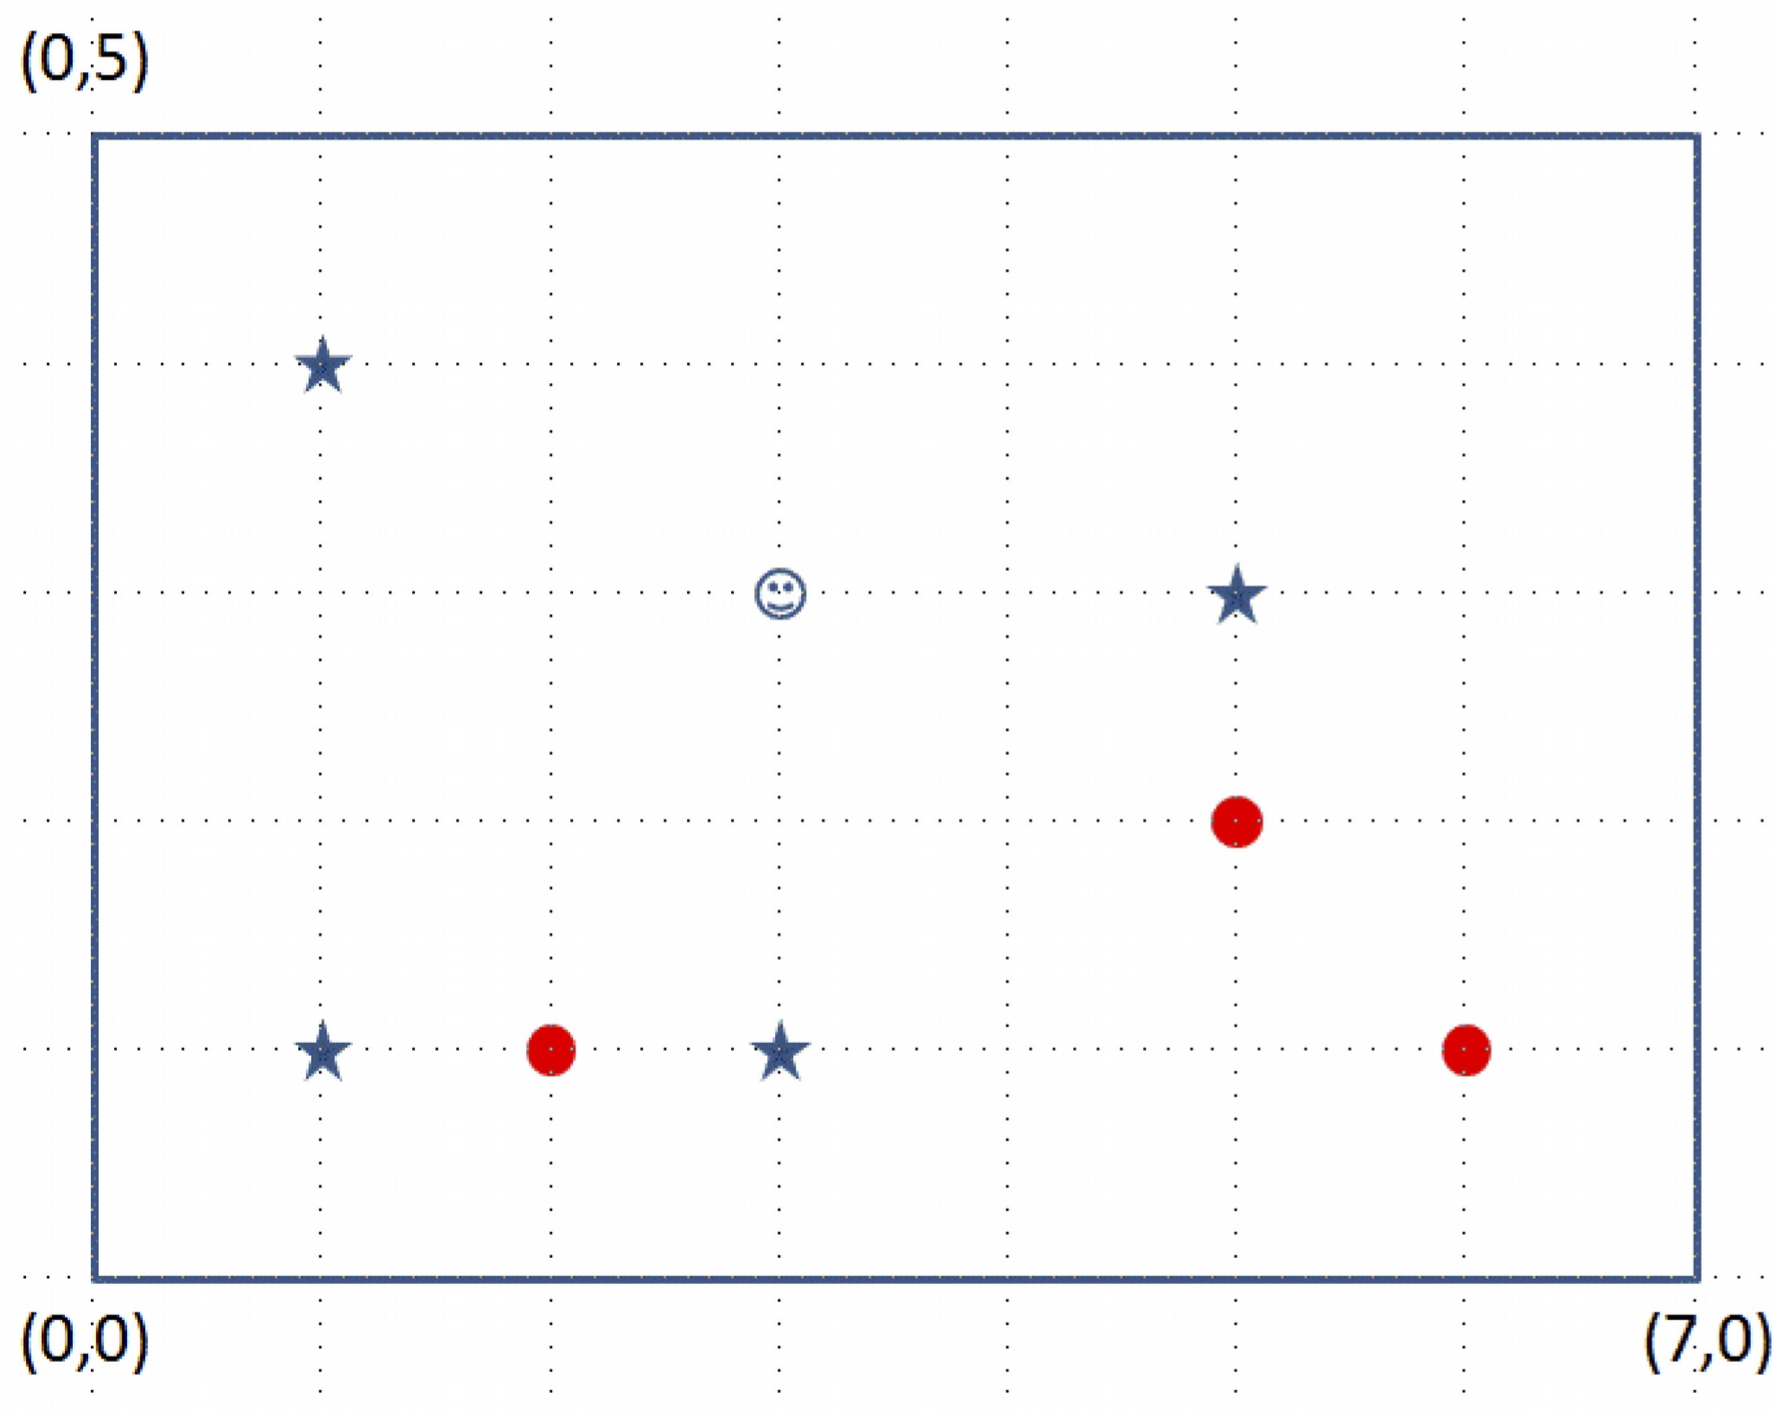
\includegraphics[width=0.5\textwidth]{exercise-1-plot}
			\end{center}
			\caption{Representación Gráfica del problema \ref{sec:e1}}
			\label{e1:plot}
		\end{figure}

		\subsection{Distancia Euclídea}

			\paragraph{}
			[TODO]

		\subsection{Distancia Euclídea Ponderada: $w_x=0.2, w_y=0.8$}

			\paragraph{}
			[TODO]

		\subsection{Distancia de Manhattan}

			\paragraph{}
			[TODO]

		\subsection{Distancia de Hamming}

			\paragraph{}
			[TODO]

	\section{Dígitos manuscritos}
	
		\paragraph{}
		[TODO]

		\begin{table}[h]
			\centering
			\small
			\begin{tabu}{ | c | c | c | c | c | c | c | c | c | c | }
				\hline
				\multicolumn{10}{ | c | }{Validación cruzada de 10 particiones --- $K$-Vecinos más Próximos} \\ \hline
				\multirow{2}{*}{Datos}	& \multicolumn{9}{ c |}{Tasa de Error ($K=$)} \\ \cline{2-10}
																& \emph{1} & \emph{2} & \emph{3} & \emph{4} & \emph{5} & \emph{6} & \emph{7} & \emph{8}	& \emph{9}\\ \hline
				Entrenae						& $3.448\%$	 & $3.524\%$ & $3.065\%$ & $3.141\%$	& $3.371\%$ & $3.218\%$	 & $3.295\%$ & $3.295\%$ & $3.371\%$	\\
				\hline
			\end{tabu}
			\caption{Tasa de error obtenida tras realizar un experimento de Validación cruzada de 10 particiones con el clasificador \emph{K-NN} para $k \in \{1,2,...,9\}$}
			\label{table:e2}
		\end{table}



		\begin{figure}[h]
			\begin{center}
				\begin{tikzpicture}
					\begin{axis}[
						% only scale the axis, not the axis including the ticks and labels
		        scale only axis=true,
		        % set `width' and `height' to the desired values
		        width=0.9\textwidth,
		        height=0.3\textwidth,
						]
						\addplot table [x=k, y=error, col sep=comma] {data.csv};
					\end{axis}
				\end{tikzpicture}
			\end{center}
			\caption{Representación Gráfica de la tasa de error obtenida tras realizar un experimento de Validación cruzada de 10 particiones con el clasificador \emph{K-NN} para $k \in \{1,2,...,9\}$}
			\label{plot:e2}
		\end{figure}

		\paragraph{}
		[TODO]


%-----------------------------
%	Bibliographic references
%-----------------------------
	\nocite{garciparedes:machine-learning-instance-based}
	\nocite{subject:taa}
	\nocite{tool:weka}
  \bibliographystyle{alpha}
  \bibliography{bib/misc}

\end{document}
